\documentclass{article}

\usepackage[utf8]{inputenc}
\usepackage{amsmath}
\usepackage{amssymb}
\usepackage{anysize}
\usepackage{color}
\usepackage{xcolor}
\usepackage{graphicx}
\usepackage{float}

\usepackage{subfigure}

\usepackage{hyperref}


\definecolor{dkgreen}{rgb}{0, 0.6, 0}
\definecolor{gray}{rgb}{0.5, 0.5, 0.5}
\usepackage{listings}
\lstset{
	language=Matlab,                	% choose the language of the code
	keywords={break,case,catch,continue,else,elseif,end,for,function,
      global,if,otherwise,persistent,return,switch,try,while},
      keywordstyle=\color{blue},
      commentstyle=\color{red},
	basicstyle=\footnotesize,       % the size of the fonts that are used for the code
	numbers= left,                 	% where to put the line-numbers
	numberstyle=\footnotesize,      % the size of the fonts that are used for the line-numbers
	stepnumber=1,                   % the step between two line-numbers. If it is 1 each line will be numbered
	numbersep=5pt,                  % how far the line-numbers are from the code
	backgroundcolor=\color{white},  % choose the background color. You must add \usepackage{color}
	showspaces=false,               % show spaces adding particular underscores
	showstringspaces=false,         % underline spaces within strings
	showtabs=false,                 % show tabs within strings adding particular underscores
	frame=single,           		% adds a frame around the code
	tabsize=2,          			% sets default tabsize to 2 spaces
	captionpos=t,          			% sets the caption-position to bottom (t=top, b=bottom)
	breaklines=true,        		% sets automatic line breaking
	breakatwhitespace=false,    	% sets if automatic breaks should only happen at whitespace
	escapeinside={\%*}{*),  % if you want to add a comment within your code
	flexiblecolumns=true}         
}

\usepackage{caption}
\DeclareCaptionFont{white}{\color{white}}
\DeclareCaptionFormat{listing}{\colorbox{gray}{\parbox[c]{\textwidth}{#1#2#3}}}
\captionsetup[lstlisting]{format=listing,labelfont=white,textfont=white}

\setlength\parindent{0pt}
\setlength{\parskip}{10pt}

\marginsize{3cm}{2cm}{2cm}{2cm}

\title{Probabilistic Robotics\\
		2D Localization Lab}
\author{Emre Ozan Alkan\\
		\{emreozanalkan@gmail.com\}\\
		MSCV-5}

\pagenumbering{arabic}
		
\date{\today}

\begin{document}
\maketitle
%\newpage




% References
% Muhammad Usman
% https://en.wikipedia.org/wiki/Robot_localization




\section{Introduction}

	Localization is main and hard to achieve task in probabilistic robotics. Localization is the problem of guessing robot's location according to external reference frame. Specific localization problems like global localization is localizing robot by only given environment map.
	
	\subsection{Environment}
	In this lab, we tried to localize robot by probabilistic method with its own uncertainty. We've given 10 by 10 grid as circular map with values 'r' and 'g' representing red and green respectively. Our robot has sensor which detecting the color of the cell of the grid. It can move up, down, right and left in the map. We also suppose to have measurement data called z:
	$$ z = [g, g, g, r, g, r, r, r, g, r] $$
Also we suppose to have movement data along with z called u:
$$u = [[0 1];
     [1 0];
     [0 1];
     [1 0];
     [1 0];
     [0 1];
     [0 1];
     [1 0];
     [1 0];
     [0 1]];$$
Where u values are:

\begin{table}[h]
\centering
\begin{tabular}{|c|c|l|l|l|}
\hline
\textbf{Robot Direction} & \multicolumn{4}{|c|}{\textbf{Representation}} \\ \hline
Left                     & \multicolumn{4}{|c|}{{[}0 -1{]}}              \\ \hline
Right                    & \multicolumn{4}{|c|}{{[}0 1{]}}               \\ \hline
Up                       & \multicolumn{4}{|c|}{{[}-1 0{]}}              \\ \hline
Down                     & \multicolumn{4}{|c|}{{[}1 0{]}}               \\ \hline
Wait                     & \multicolumn{4}{|c|}{{[}0 0{]}}               \\ \hline
\end{tabular}
\end{table}

\par Since in real world, there is no certainty, we also need to keep track of our uncertainty. Thus, we have $ pHit $ representing correct sensor read. Whereas we also have $ pMiss $ representing probability of wrong sensor reading. Their values are 0.7 and 0.3, respectively. 

\par On the other hand, robot movement is also not perfect in real world, hence, we should keep track of its uncertainty too. So we keep $ pMove, pUndershoot and pOvershoot $ with respective 0.8, 0.1 and 0.1 probabilities, representing probabilities of correct movement, less movement or more movement.

\section{Implementation}
\par We implemented 2 functions in Matlab. Sense function - takes prior probability and measurement and find posterior probability, Move function - taking prior, motion and uncertainty as input and find prediction to update measurements. Here are implementations:

\begin{lstlisting}[label=main-m, caption=Main.m]
	
close all;
clear all;
clc;

worldWidth = 10;
worldHeight = 10;

world = [ 'r', 'g', 'g', 'r', 'r', 'r', 'g', 'g', 'r', 'r';
          'r', 'r', 'g', 'r', 'r', 'r', 'r', 'g', 'r', 'r';
          'r', 'r', 'g', 'g', 'r', 'r', 'r', 'g', 'g', 'r';
          'r', 'r', 'r', 'r', 'r', 'r', 'r', 'r', 'r', 'r';
          'g', 'g', 'g', 'g', 'g', 'g', 'g', 'g', 'g', 'g';
          'r', 'g', 'g', 'r', 'r', 'r', 'g', 'g', 'r', 'r';
          'r', 'r', 'g', 'r', 'r', 'r', 'r', 'g', 'r', 'r';
          'r', 'r', 'g', 'g', 'r', 'r', 'r', 'g', 'g', 'r';
          'r', 'r', 'r', 'r', 'r', 'r', 'r', 'r', 'r', 'r';
          'g', 'g', 'g', 'g', 'g', 'g', 'g', 'g', 'g', 'g'];

worldProbabilty = ones(worldWidth, worldHeight) ./ (worldWidth * worldHeight);
imagesc(worldProbabilty); title('Prior Probability of World');

z = ['g', 'g', 'g', 'r', 'g', 'r', 'r', 'r', 'g', 'r'];

pHit = 0.7;
pMiss = 0.3;

pMove = 0.8;
pUndershoot = 0.1;
pOvershoot = 0.1;

u = [[0 1];
     [1 0];
     [0 1];
     [1 0];
     [1 0];
     [0 1];
     [0 1];
     [1 0];
     [1 0];
     [0 1]];
 
 
pathCount = numel(z);

for ii = 1 : pathCount
    
    worldProbabilty = sense(worldProbabilty, z(ii), pHit, pMiss, world);
    
    worldProbabilty = move(worldProbabilty, u(ii, :), pMove, pOvershoot, pUndershoot);
    
end

pause(2);

imagesc(worldProbabilty); title('Posterior Probability of World');

\end{lstlisting}
\newpage
\begin{lstlisting}[label=sense-m, caption=sense.m]
	
function [ q ] = sense(p, z, pHit, pMiss, world)

[m, n] = size(p);

q = ones(m, n);

for ii = 1 : m
    
    for jj = 1 : n
        
        if strcmp(world(ii, jj), z)
            q(ii, jj) = pHit * p(ii, jj);
        else
            q(ii, jj) = pMiss * p(ii, jj);
        end
        
    end
    
end

q = q / sum(q(:));

end

\end{lstlisting}


\begin{lstlisting}[label=move-m, caption=move.m]
	
function [ q ] = move(p, u, pCorrect, pOvershooting, pUndershooting)

qCorrect = pCorrect * circshift(p, u);

qOvershooting = pOvershooting * circshift(p, u + 1);

qUndershooting = pUndershooting * circshift(p, u - 1);

q = qCorrect + qOvershooting + qUndershooting;

end

\end{lstlisting}


\section{Results}

Since world is 10 by 10 grid, contains 100 elements, all of its grid elements were having 0.01 probability initially. After robot starts to move, with sensing and moving, it tries to locate its belief, uncertainty, into more compound in other word less uncertain condition. After running the code, here is the results of the 10 by 10 map, indicating 4 different peaks that our robot more likely to be. Since this map is recurrent, of 4 individual square, robot is more likely to be in one of the peak of this 4 individual repetitive patterns. 

\begin{figure}[H]
\begin{center}
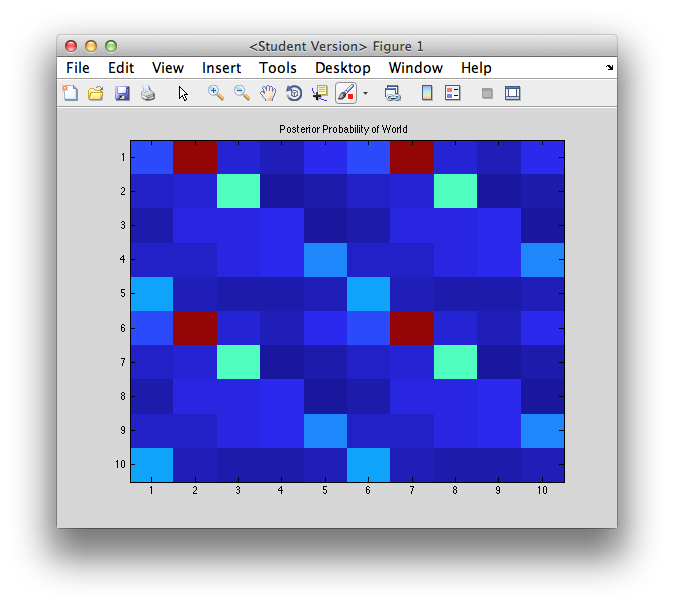
\includegraphics[scale=0.6]{2DLocalizationResult.png}
\caption{Posterior Probability of World}
\end{center}
\end{figure}	


\section{References}
\begin{enumerate}
	\item \href{url}{http://www.probabilistic-robotics.org/}
\end{enumerate}


\end{document}